\section{Variable Bias Voltage SRF Temperature Fit Residuals}
%============================================================
\label{app:Vset_tfit_data_plots}

\subsection{Channel 1}
\begin{figure}[H]
  \label{fig:Vset.ch1_tfit}
  \centering
  \includegraphics[scale=0.45]{graphics/tfit/Vset/atms_npp-1.tfit.eps}
  \caption{ATMS channel 1 polychromatic correction temperature fit residuals at nominal temperature (20\textdegree{}C) for the three test voltages: $V_{NOM}$, $V_{LO}$, and $V_{HI}$.}
\end{figure}

\subsection{Channel 2}
\begin{figure}[H]
  \label{fig:Vset.ch2_tfit}
  \centering
  \includegraphics[scale=0.45]{graphics/tfit/Vset/atms_npp-2.tfit.eps}
  \caption{ATMS channel 2 polychromatic correction temperature fit residuals at nominal temperature (20\textdegree{}C) for the three test voltages: $V_{NOM}$, $V_{LO}$, and $V_{HI}$.}
\end{figure}

\subsection{Channel 3}
\begin{figure}[H]
  \label{fig:Vset.ch3_tfit}
  \centering
  \includegraphics[scale=0.45]{graphics/tfit/Vset/atms_npp-3.tfit.eps}
  \caption{ATMS channel 3 polychromatic correction temperature fit residuals at nominal temperature (20\textdegree{}C) for the three test voltages: $V_{NOM}$, $V_{LO}$, and $V_{HI}$.}
\end{figure}

\subsection{Channel 4}
\begin{figure}[H]
  \label{fig:Vset.ch4_tfit}
  \centering
  \includegraphics[scale=0.45]{graphics/tfit/Vset/atms_npp-4.tfit.eps}
  \caption{ATMS channel 4 polychromatic correction temperature fit residuals at nominal temperature (20\textdegree{}C) for the three test voltages: $V_{NOM}$, $V_{LO}$, and $V_{HI}$.}
\end{figure}

\subsection{Channel 5}
\begin{figure}[H]
  \label{fig:Vset.ch5_tfit}
  \centering
  \includegraphics[scale=0.45]{graphics/tfit/Vset/atms_npp-5.tfit.eps}
  \caption{ATMS channel 5 polychromatic correction temperature fit residuals at nominal temperature (20\textdegree{}C) for the three test voltages: $V_{NOM}$, $V_{LO}$, and $V_{HI}$.}
\end{figure}

\subsection{Channel 6}
\begin{figure}[H]
  \label{fig:Vset.ch6_tfit}
  \centering
  \includegraphics[scale=0.45]{graphics/tfit/Vset/atms_npp-6.tfit.eps}
  \caption{ATMS channel 6 polychromatic correction temperature fit residuals at nominal temperature (20\textdegree{}C) for the three test voltages: $V_{NOM}$, $V_{LO}$, and $V_{HI}$.}
\end{figure}

\subsection{Channel 7}
\begin{figure}[H]
  \label{fig:Vset.ch7_tfit}
  \centering
  \includegraphics[scale=0.45]{graphics/tfit/Vset/atms_npp-7.tfit.eps}
  \caption{ATMS channel 7 polychromatic correction temperature fit residuals at nominal temperature (20\textdegree{}C) for the three test voltages: $V_{NOM}$, $V_{LO}$, and $V_{HI}$.}
\end{figure}

\subsection{Channel 8}
\begin{figure}[H]
  \label{fig:Vset.ch8_tfit}
  \centering
  \includegraphics[scale=0.45]{graphics/tfit/Vset/atms_npp-8.tfit.eps}
  \caption{ATMS channel 8 polychromatic correction temperature fit residuals at nominal temperature (20\textdegree{}C) for the three test voltages: $V_{NOM}$, $V_{LO}$, and $V_{HI}$.}
\end{figure}

\subsection{Channel 9}
\begin{figure}[H]
  \label{fig:Vset.ch9_tfit}
  \centering
  \includegraphics[scale=0.45]{graphics/tfit/Vset/atms_npp-9.tfit.eps}
  \caption{ATMS channel 9 polychromatic correction temperature fit residuals at nominal temperature (20\textdegree{}C) for the three test voltages: $V_{NOM}$, $V_{LO}$, and $V_{HI}$.}
\end{figure}

\subsection{Channel 10}
\begin{figure}[H]
  \label{fig:Vset.ch10_tfit}
  \centering
  \includegraphics[scale=0.45]{graphics/tfit/Vset/atms_npp-10.tfit.eps}
  \caption{ATMS channel 10 polychromatic correction temperature fit residuals at nominal temperature (20\textdegree{}C) for the three test voltages: $V_{NOM}$, $V_{LO}$, and $V_{HI}$.}
\end{figure}

\subsection{Channel 11}
\begin{figure}[H]
  \label{fig:Vset.ch11_tfit}
  \centering
  \includegraphics[scale=0.45]{graphics/tfit/Vset/atms_npp-11.tfit.eps}
  \caption{ATMS channel 11 polychromatic correction temperature fit residuals at nominal temperature (20\textdegree{}C) for the three test voltages: $V_{NOM}$, $V_{LO}$, and $V_{HI}$.}
\end{figure}

\subsection{Channel 12}
\begin{figure}[H]
  \label{fig:Vset.ch12_tfit}
  \centering
  \includegraphics[scale=0.45]{graphics/tfit/Vset/atms_npp-12.tfit.eps}
  \caption{ATMS channel 12 polychromatic correction temperature fit residuals at nominal temperature (20\textdegree{}C) for the three test voltages: $V_{NOM}$, $V_{LO}$, and $V_{HI}$.}
\end{figure}

\subsection{Channel 13}
\begin{figure}[H]
  \label{fig:Vset.ch13_tfit}
  \centering
  \includegraphics[scale=0.45]{graphics/tfit/Vset/atms_npp-13.tfit.eps}
  \caption{ATMS channel 13 polychromatic correction temperature fit residuals at nominal temperature (20\textdegree{}C) for the three test voltages: $V_{NOM}$, $V_{LO}$, and $V_{HI}$.}
\end{figure}

\subsection{Channel 14}
\begin{figure}[H]
  \label{fig:Vset.ch14_tfit}
  \centering
  \includegraphics[scale=0.45]{graphics/tfit/Vset/atms_npp-14.tfit.eps}
  \caption{ATMS channel 14 polychromatic correction temperature fit residuals at nominal temperature (20\textdegree{}C) for the three test voltages: $V_{NOM}$, $V_{LO}$, and $V_{HI}$.}
\end{figure}

\subsection{Channel 15}
\begin{figure}[H]
  \label{fig:Vset.ch15_tfit}
  \centering
  \includegraphics[scale=0.45]{graphics/tfit/Vset/atms_npp-15.tfit.eps}
  \caption{ATMS channel 15 polychromatic correction temperature fit residuals at nominal temperature (20\textdegree{}C) for the three test voltages: $V_{NOM}$, $V_{LO}$, and $V_{HI}$.}
\end{figure}

\subsection{Channel 16}
\begin{figure}[H]
  \label{fig:Vset.ch16_tfit}
  \centering
  \includegraphics[scale=0.45]{graphics/tfit/Vset/atms_npp-16.tfit.eps}
  \caption{ATMS channel 16 polychromatic correction temperature fit residuals at nominal temperature (20\textdegree{}C) for the three test voltages: $V_{NOM}$, $V_{LO}$, and $V_{HI}$.}
\end{figure}

\subsection{Channel 17}
\begin{figure}[H]
  \label{fig:Vset.ch17_tfit}
  \centering
  \includegraphics[scale=0.45]{graphics/tfit/Vset/atms_npp-17.tfit.eps}
  \caption{ATMS channel 17 polychromatic correction temperature fit residuals at nominal temperature (20\textdegree{}C) for the three test voltages: $V_{NOM}$, $V_{LO}$, and $V_{HI}$.}
\end{figure}

\subsection{Channel 18}
\begin{figure}[H]
  \label{fig:Vset.ch18_tfit}
  \centering
  \includegraphics[scale=0.45]{graphics/tfit/Vset/atms_npp-18.tfit.eps}
  \caption{ATMS channel 18 polychromatic correction temperature fit residuals at nominal temperature (20\textdegree{}C) for the three test voltages: $V_{NOM}$, $V_{LO}$, and $V_{HI}$.}
\end{figure}

\subsection{Channel 19}
\begin{figure}[H]
  \label{fig:Vset.ch19_tfit}
  \centering
  \includegraphics[scale=0.45]{graphics/tfit/Vset/atms_npp-19.tfit.eps}
  \caption{ATMS channel 19 polychromatic correction temperature fit residuals at nominal temperature (20\textdegree{}C) for the three test voltages: $V_{NOM}$, $V_{LO}$, and $V_{HI}$.}
\end{figure}

\subsection{Channel 20}
\begin{figure}[H]
  \label{fig:Vset.ch20_tfit}
  \centering
  \includegraphics[scale=0.45]{graphics/tfit/Vset/atms_npp-20.tfit.eps}
  \caption{ATMS channel 20 polychromatic correction temperature fit residuals at nominal temperature (20\textdegree{}C) for the three test voltages: $V_{NOM}$, $V_{LO}$, and $V_{HI}$.}
\end{figure}

\subsection{Channel 21}
\begin{figure}[H]
  \label{fig:Vset.ch21_tfit}
  \centering
  \includegraphics[scale=0.45]{graphics/tfit/Vset/atms_npp-21.tfit.eps}
  \caption{ATMS channel 21 polychromatic correction temperature fit residuals at nominal temperature (20\textdegree{}C) for the three test voltages: $V_{NOM}$, $V_{LO}$, and $V_{HI}$.}
\end{figure}

\subsection{Channel 22}
\begin{figure}[H]
  \label{fig:Vset.ch22_tfit}
  \centering
  \includegraphics[scale=0.45]{graphics/tfit/Vset/atms_npp-22.tfit.eps}
  \caption{ATMS channel 22 polychromatic correction temperature fit residuals at nominal temperature (20\textdegree{}C) for the three test voltages: $V_{NOM}$, $V_{LO}$, and $V_{HI}$.}
\end{figure}
